\documentclass[11pt]{article}

\usepackage{float}
\usepackage{hyperref}
\usepackage{fullpage}
\usepackage{verbatim}
\usepackage{moreverb}
\usepackage{graphicx}
\usepackage{parskip}
\usepackage{amsmath}
\usepackage[toc,page]{appendix}
\graphicspath{{images/}}
\usepackage{gensymb}

\usepackage{minted}
\let\verbatiminput=\verbatimtabinput
\def\verbatimtabsize{4\relax}

\begin{document}
\title{EE 241B HW3 Writeup}

\author{Vighnesh Iyer}
\date{}
\maketitle

\tableofcontents

\section{Building and Characterizing a Standard Cell}

\subsection{Flow and Decoder Delay Using Custom Cell}
We go through the tutorial to design a custom NAND2 standard cell. We first record the critical path of the 3-8 decoder used in the previous lab with the NAND2 cell supplied with the design kit. The critical path goes from \verb|A[3]| to \verb|Z[5]| and it has a delay of 0.1376 ns.

We then tell DC and ICC to use our custom standard cell and we measure the critical path again. The critical path now goes from \verb|A[0]| to \verb|Z[14]| and has a delay of 0.1019 ns, which is an improvement over the previous ICC run. However, looking at the final Verilog netlist from ICC only 2 instances of our \verb|NAND2X1B_RVT| cell exist. However, after running only DC, there were many instances of our custom cell. It seems that ICC did some optimization and swapped out most of those custom cells for standard cells from the design kit.

\begin{figure}[H]
	\centerline{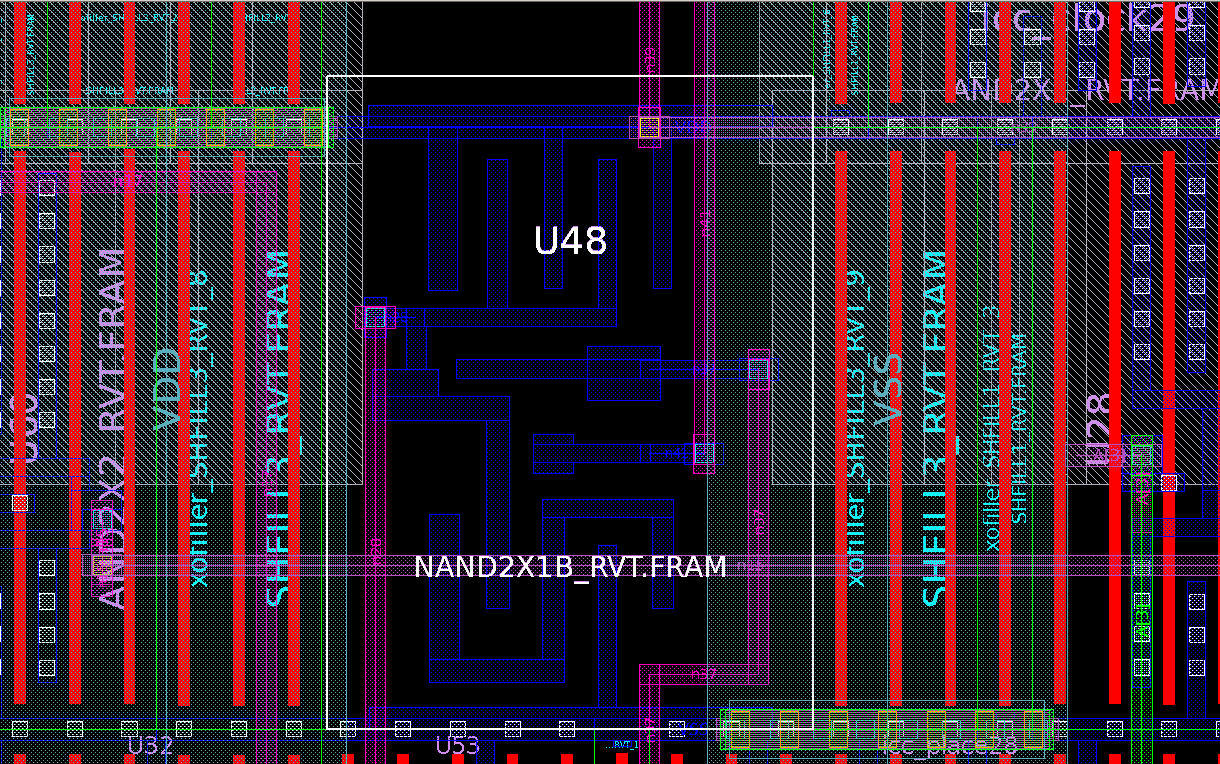
\includegraphics[height=7cm]{icc_custom_cell.png}}
	\caption{An instance of the NAND2X1B\_RVT cell in ICC with visible M1 polygons.}
\end{figure}

\subsection{Standard Cell Inverter Variation Impact vs $V_{DD}$}
We run a 300 point Monte Carlo simulation and plot the mean and sigma for the input-rising/output-falling delay of the \verb|INVX0_RVT| standard cell for $V_{DD}$ between 0.2 and 1.05. We fix an input slope of 10ps and a 1fF load. This part was done by exporting a netlist from Virtuoso and using commandline HSPICE for the simulation.

\begin{figure}[H]
	\centerline{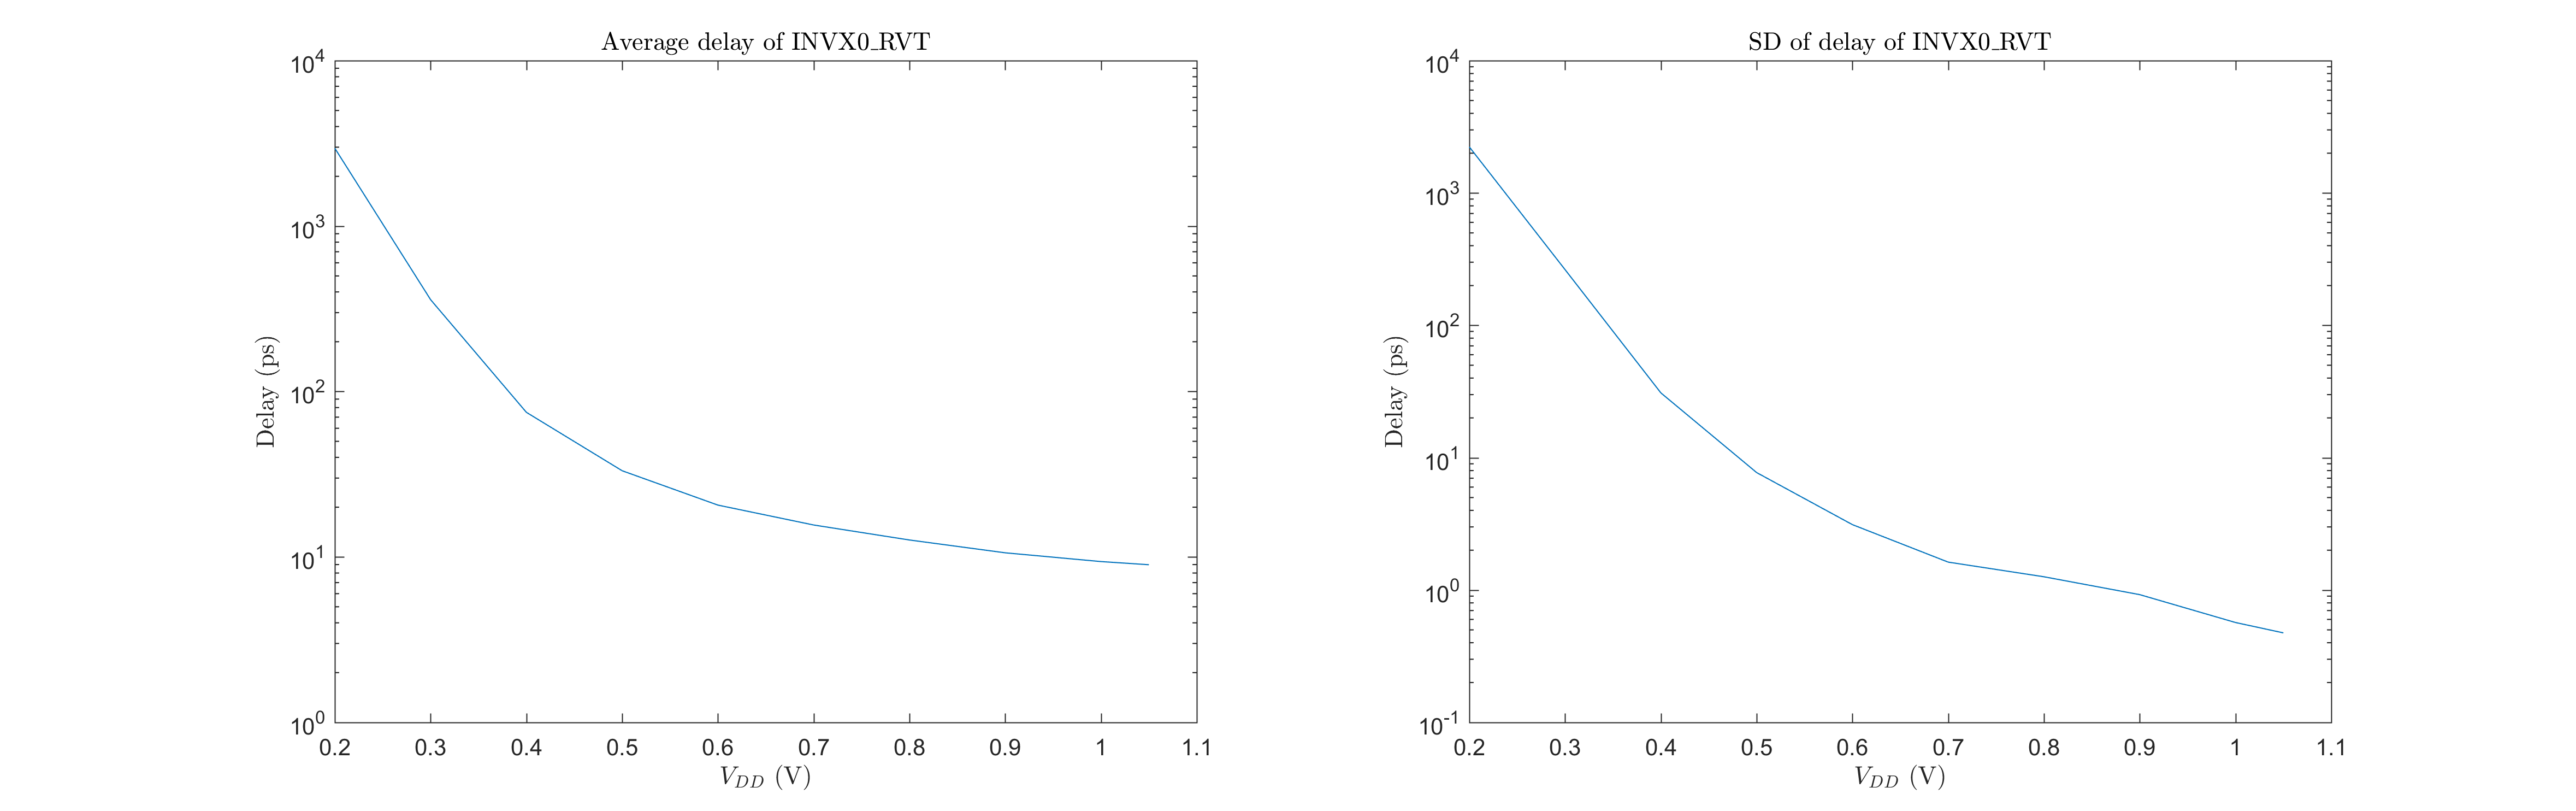
\includegraphics[width=\textwidth+4cm]{delay_vs_vdd.png}}
	\caption{Plot is log-scale in y-axis.}
\end{figure}

We then plot $\sigma / \mu$ vs. $V_{DD}$.

\begin{figure}[H]
	\centerline{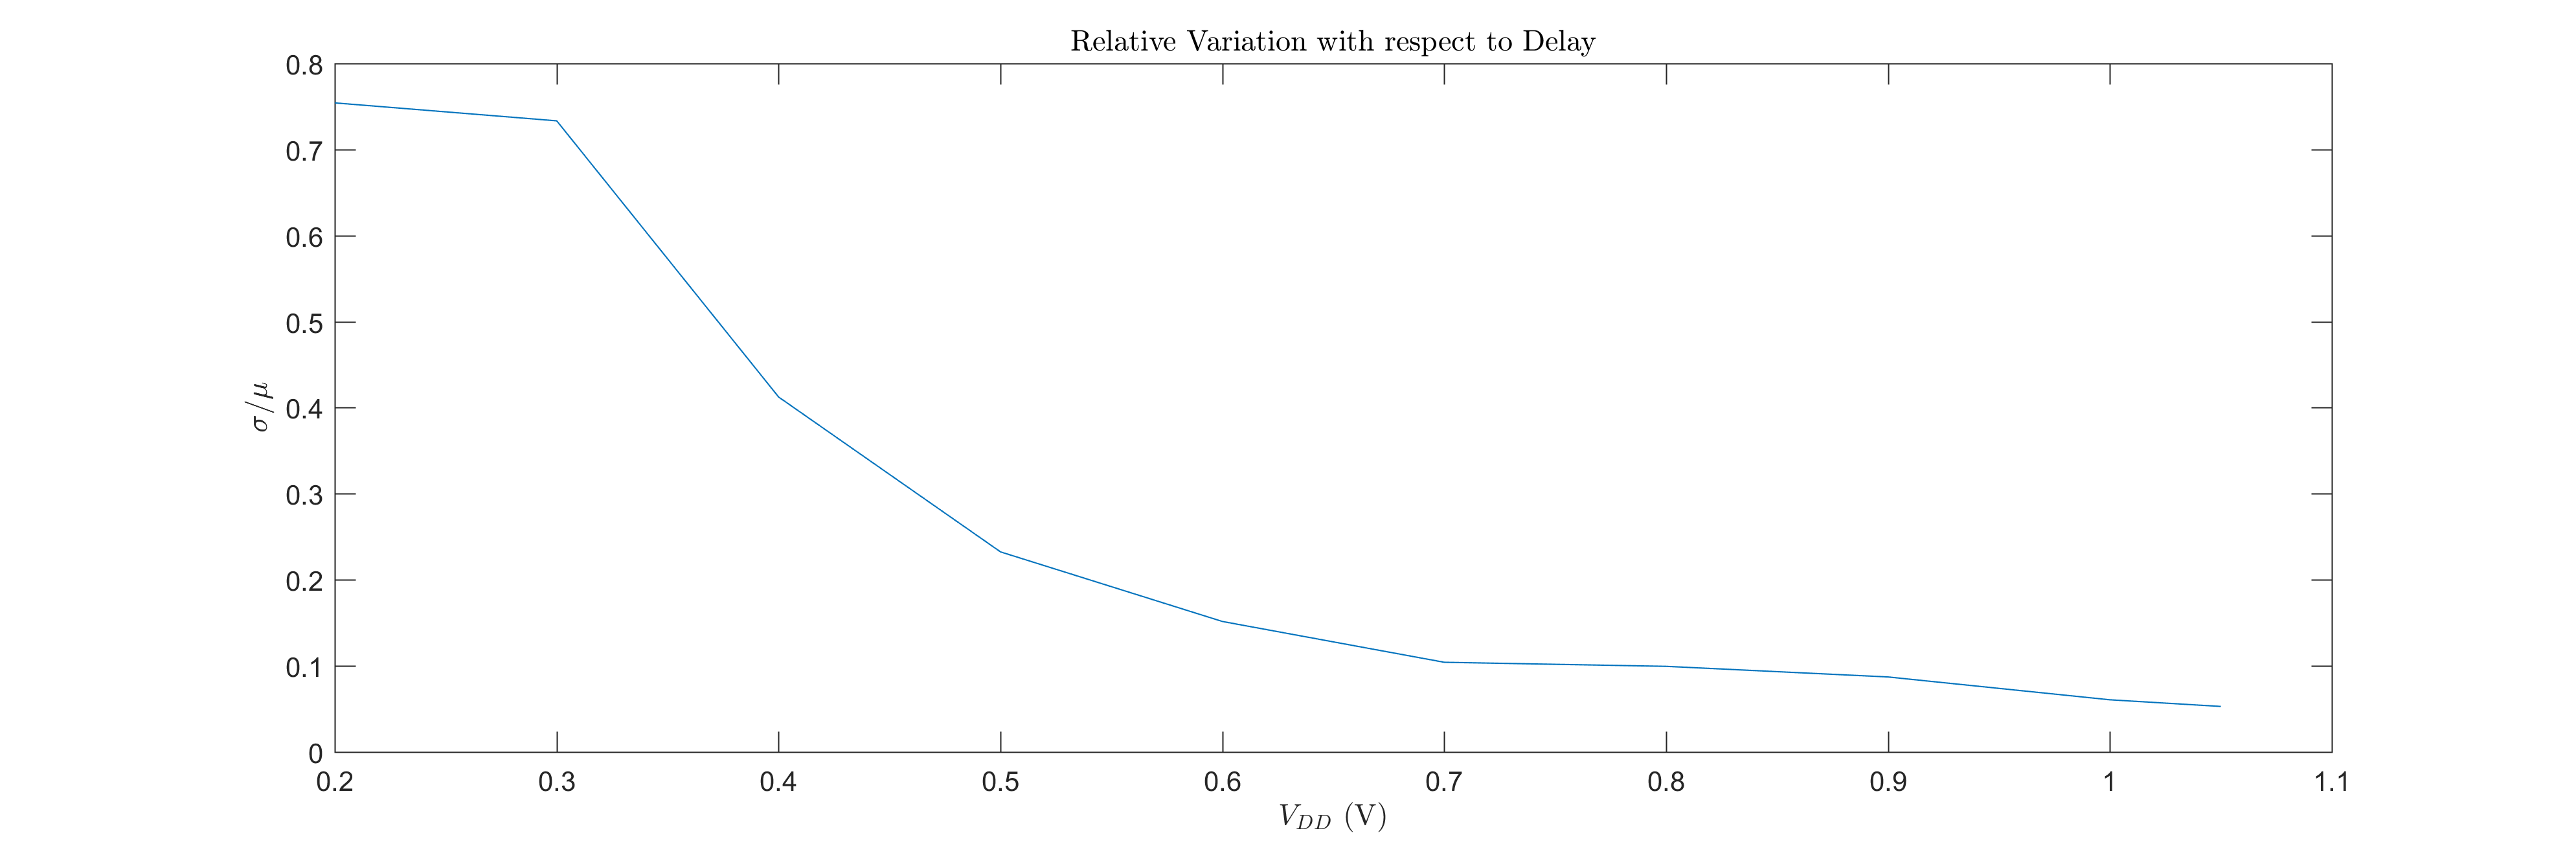
\includegraphics[width=\textwidth+4cm]{relative_delay_variation_vs_vdd.png}}
\end{figure}

Finally we plot the delay of a $6 \sigma$ cell relative to the mean vs. $V_{DD}$.


\section{Flip-Flops}
\begin{figure}[H]
	\centerline{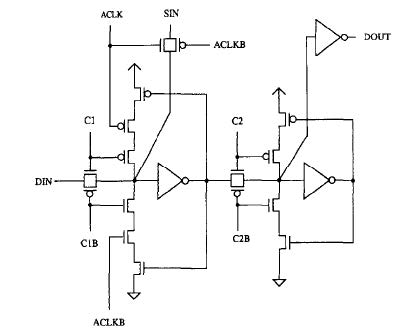
\includegraphics[height=5cm]{flip_flop_schematic.jpg}}
	\caption{A schematic of a sequential circuit.}
\end{figure}

\subsection{Identify Circuit}

Assuming that C1 and C2 are opposite phases of the same clock, the circuit above implements a \textbf{D-type flip-flop} using a master-slave latch topology.

When C1 is high, the first transmission gate is transparent and the data is allowed to settle at the input of the second transmission gate. At the moment that C2 goes high, C1 goes low to close off any further input changes, and the output reflects the 'last' value that passed through the first transmission gate while C1 was high.

The rest of the circuitry serves to make the flip-flop static by providing feedback into the storage nodes and there is an additional transmission gate that can be used by a scan chain.

\subsection{FF Timing Characteristics}
Assuming that the NMOS and PMOS devices have the same mobility and are all symmetrically sized, order the following timing parameters by magnitude: setup time, hold time, clock-output delay.

The setup time is approximately equal to the time it takes for an input signal at \verb|DIN| to race past the first transmission gate, after which the gate can become opaque. The hold time is close to 0 since after C2 goes high

\newpage
\appendix

\end{document}